% Electrical Circuit Progress Report - Deployment System
\documentclass[12pt]{article}
\usepackage[margin=1in]{geometry}
\usepackage{graphicx}
\usepackage{caption}
\usepackage{float}

\title{Electrical Circuit Progress Report\\Deployment System}
\author{0104C}
\date{\today}

\begin{document}

\maketitle

\section{Introduction}

This report documents the development of the electrical circuit for the deployment system. The circuit integrates servo motors with a microcontroller to enable controlled deployment functionality. The build process adapts foundational concepts from Lab 3 and incorporates additional components to meet the specific requirements of the deployment mechanism. The following circuit schematic was followed in the build of the final iteration of the deployment circuit:

\begin{figure}[H]
\centering
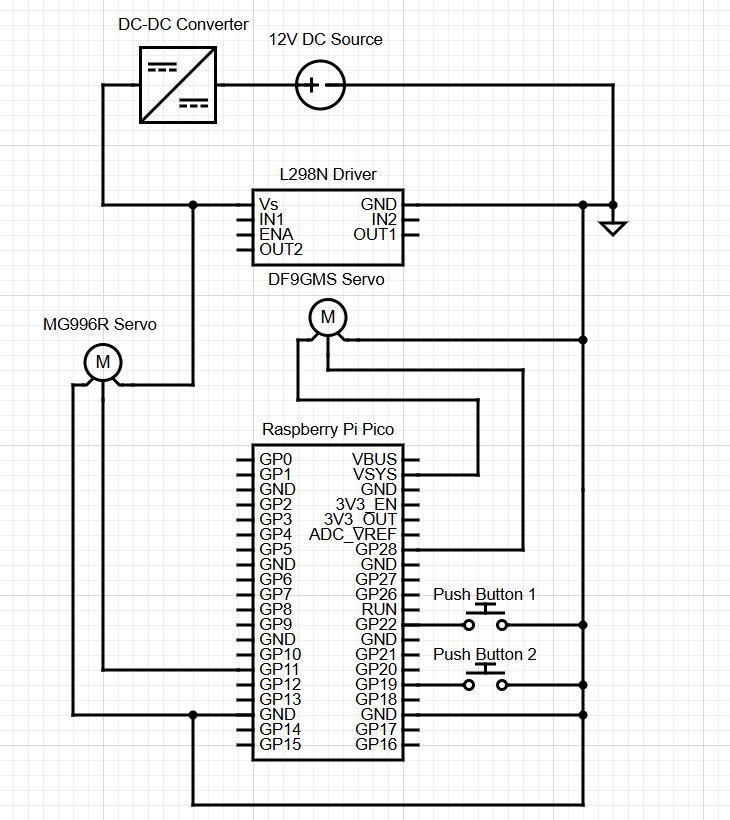
\includegraphics[width=0.60\textwidth]{../circuit_diagram_deployment.png}
\caption{Circuit schematic for the deployment system.}
\label{fig:circuit}
\end{figure}

\section{Circuit Development Progress}

\subsection{Initial Setup}

The circuit development began by adapting the Lab 3 circuit design as outlined in the 04.1.1 Deployment Electrical Subsystem Deployment Report. Figure \ref{fig:initial} shows the initial configuration, which includes the microcontroller on a breadboard, buck converter module, motor driver board, and a single test servo motor. This setup established the basic power distribution and control logic framework.

\begin{figure}[H]
\centering
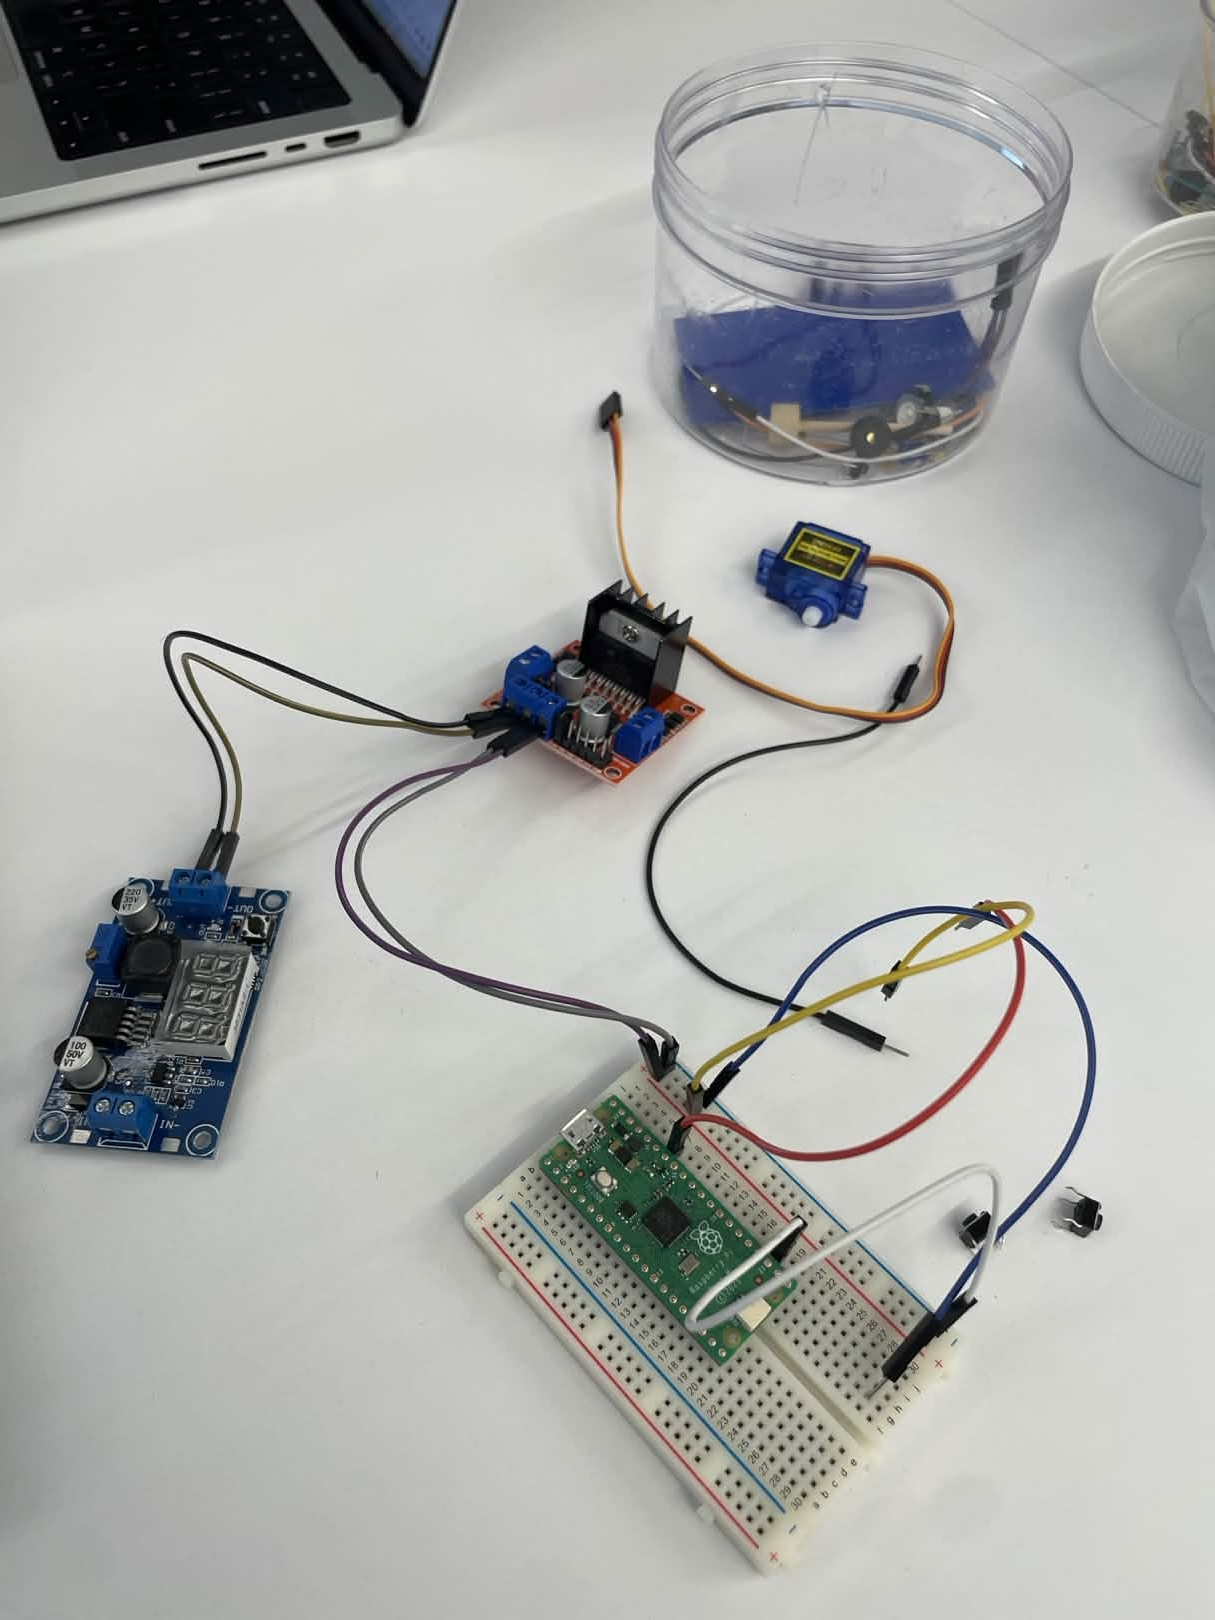
\includegraphics[width=0.75\textwidth]{../electrical_images/initial_setup.jpg}
\caption{Initial circuit setup adapted from Lab 3, showing microcontroller, buck converter, motor driver, and test servo.}
\label{fig:initial}
\end{figure}

\subsection{Power Configuration}

Figure \ref{fig:power} demonstrates the detailed power wiring configuration. The buck converter regulates the input voltage to the appropriate level for the servo motors, while the motor drivers provide the necessary current amplification. Power and ground connections were carefully routed to ensure stable operation of the servo motors under load.

\begin{figure}[H]
\centering
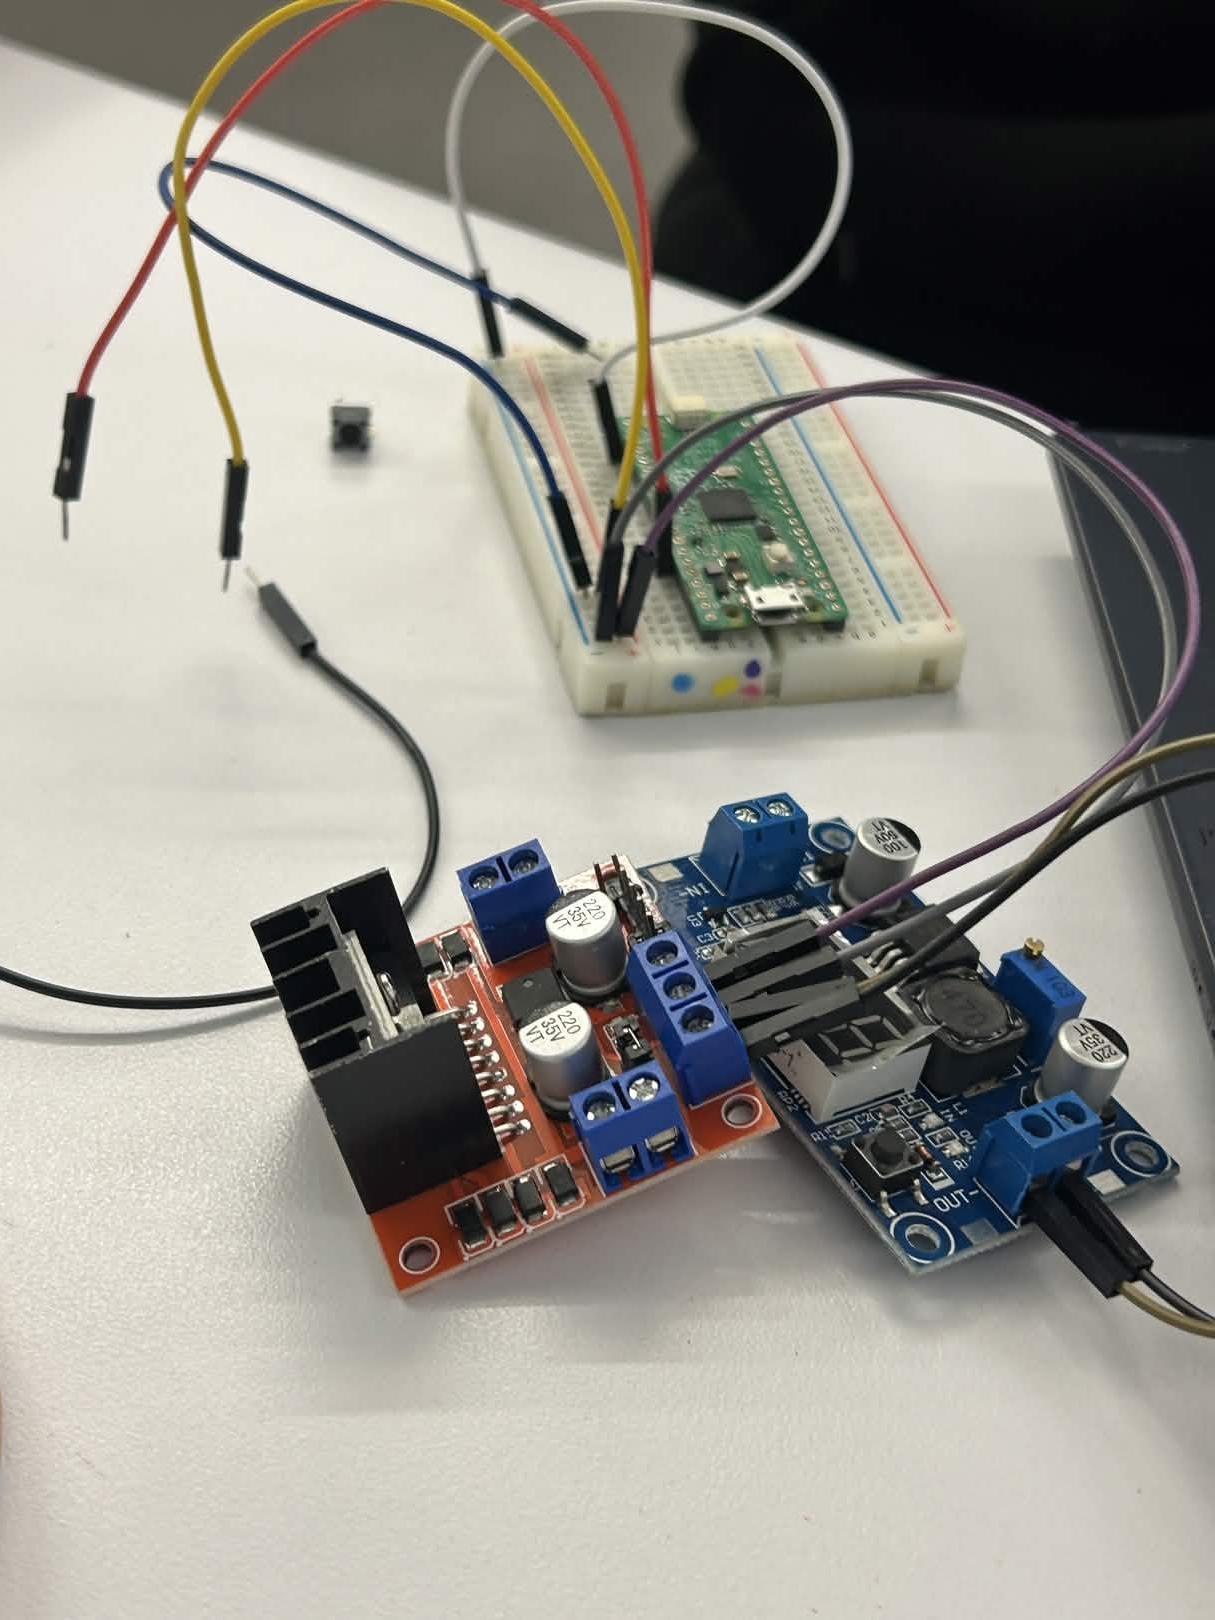
\includegraphics[width=0.75\textwidth]{../electrical_images/power_setup.jpg}
\caption{Detailed power setup showing buck converter and motor driver wiring for servo power delivery.}
\label{fig:power}
\end{figure}

\subsection{Servo Integration}

The servo motors were integrated into the circuit board as shown in Figure \ref{fig:building}. Each servo was connected with three wires: power, ground, and signal. The power and ground lines were connected to the regulated power supply, while the signal wires were routed to the logic pins of the microcontroller to enable PWM control of the servo positions.

\begin{figure}[H]
\centering
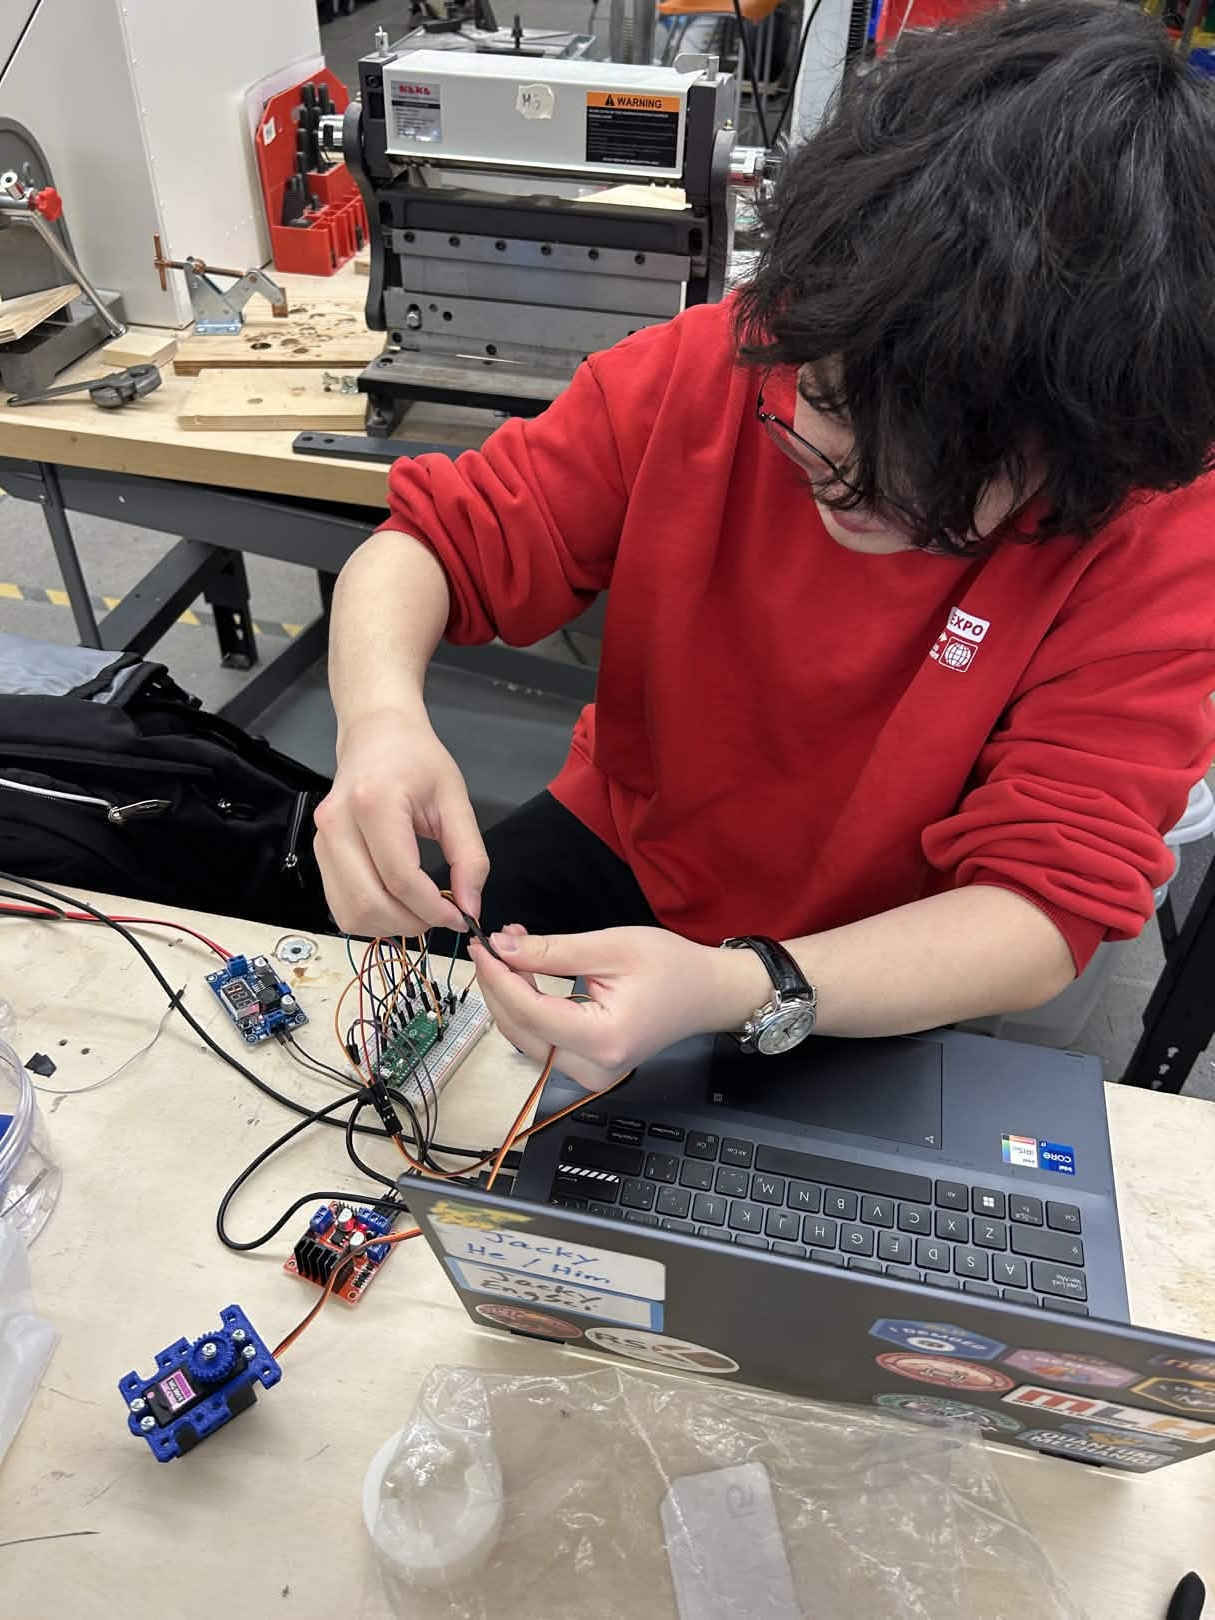
\includegraphics[width=0.75\textwidth]{../electrical_images/building_servo.jpg}
\caption{Servo integration process showing connection of power, ground, and signal lines to the circuit board.}
\label{fig:building}
\end{figure}

\subsection{Final Integrated System}

Figure \ref{fig:final} shows the completed circuit with all components integrated. The final configuration includes two servo motors and two push buttons. The push buttons provide manual control inputs, with each button mapped to control one of the two servos. This setup enables testing and demonstration of the deployment mechanism functionality.

\begin{figure}[H]
\centering
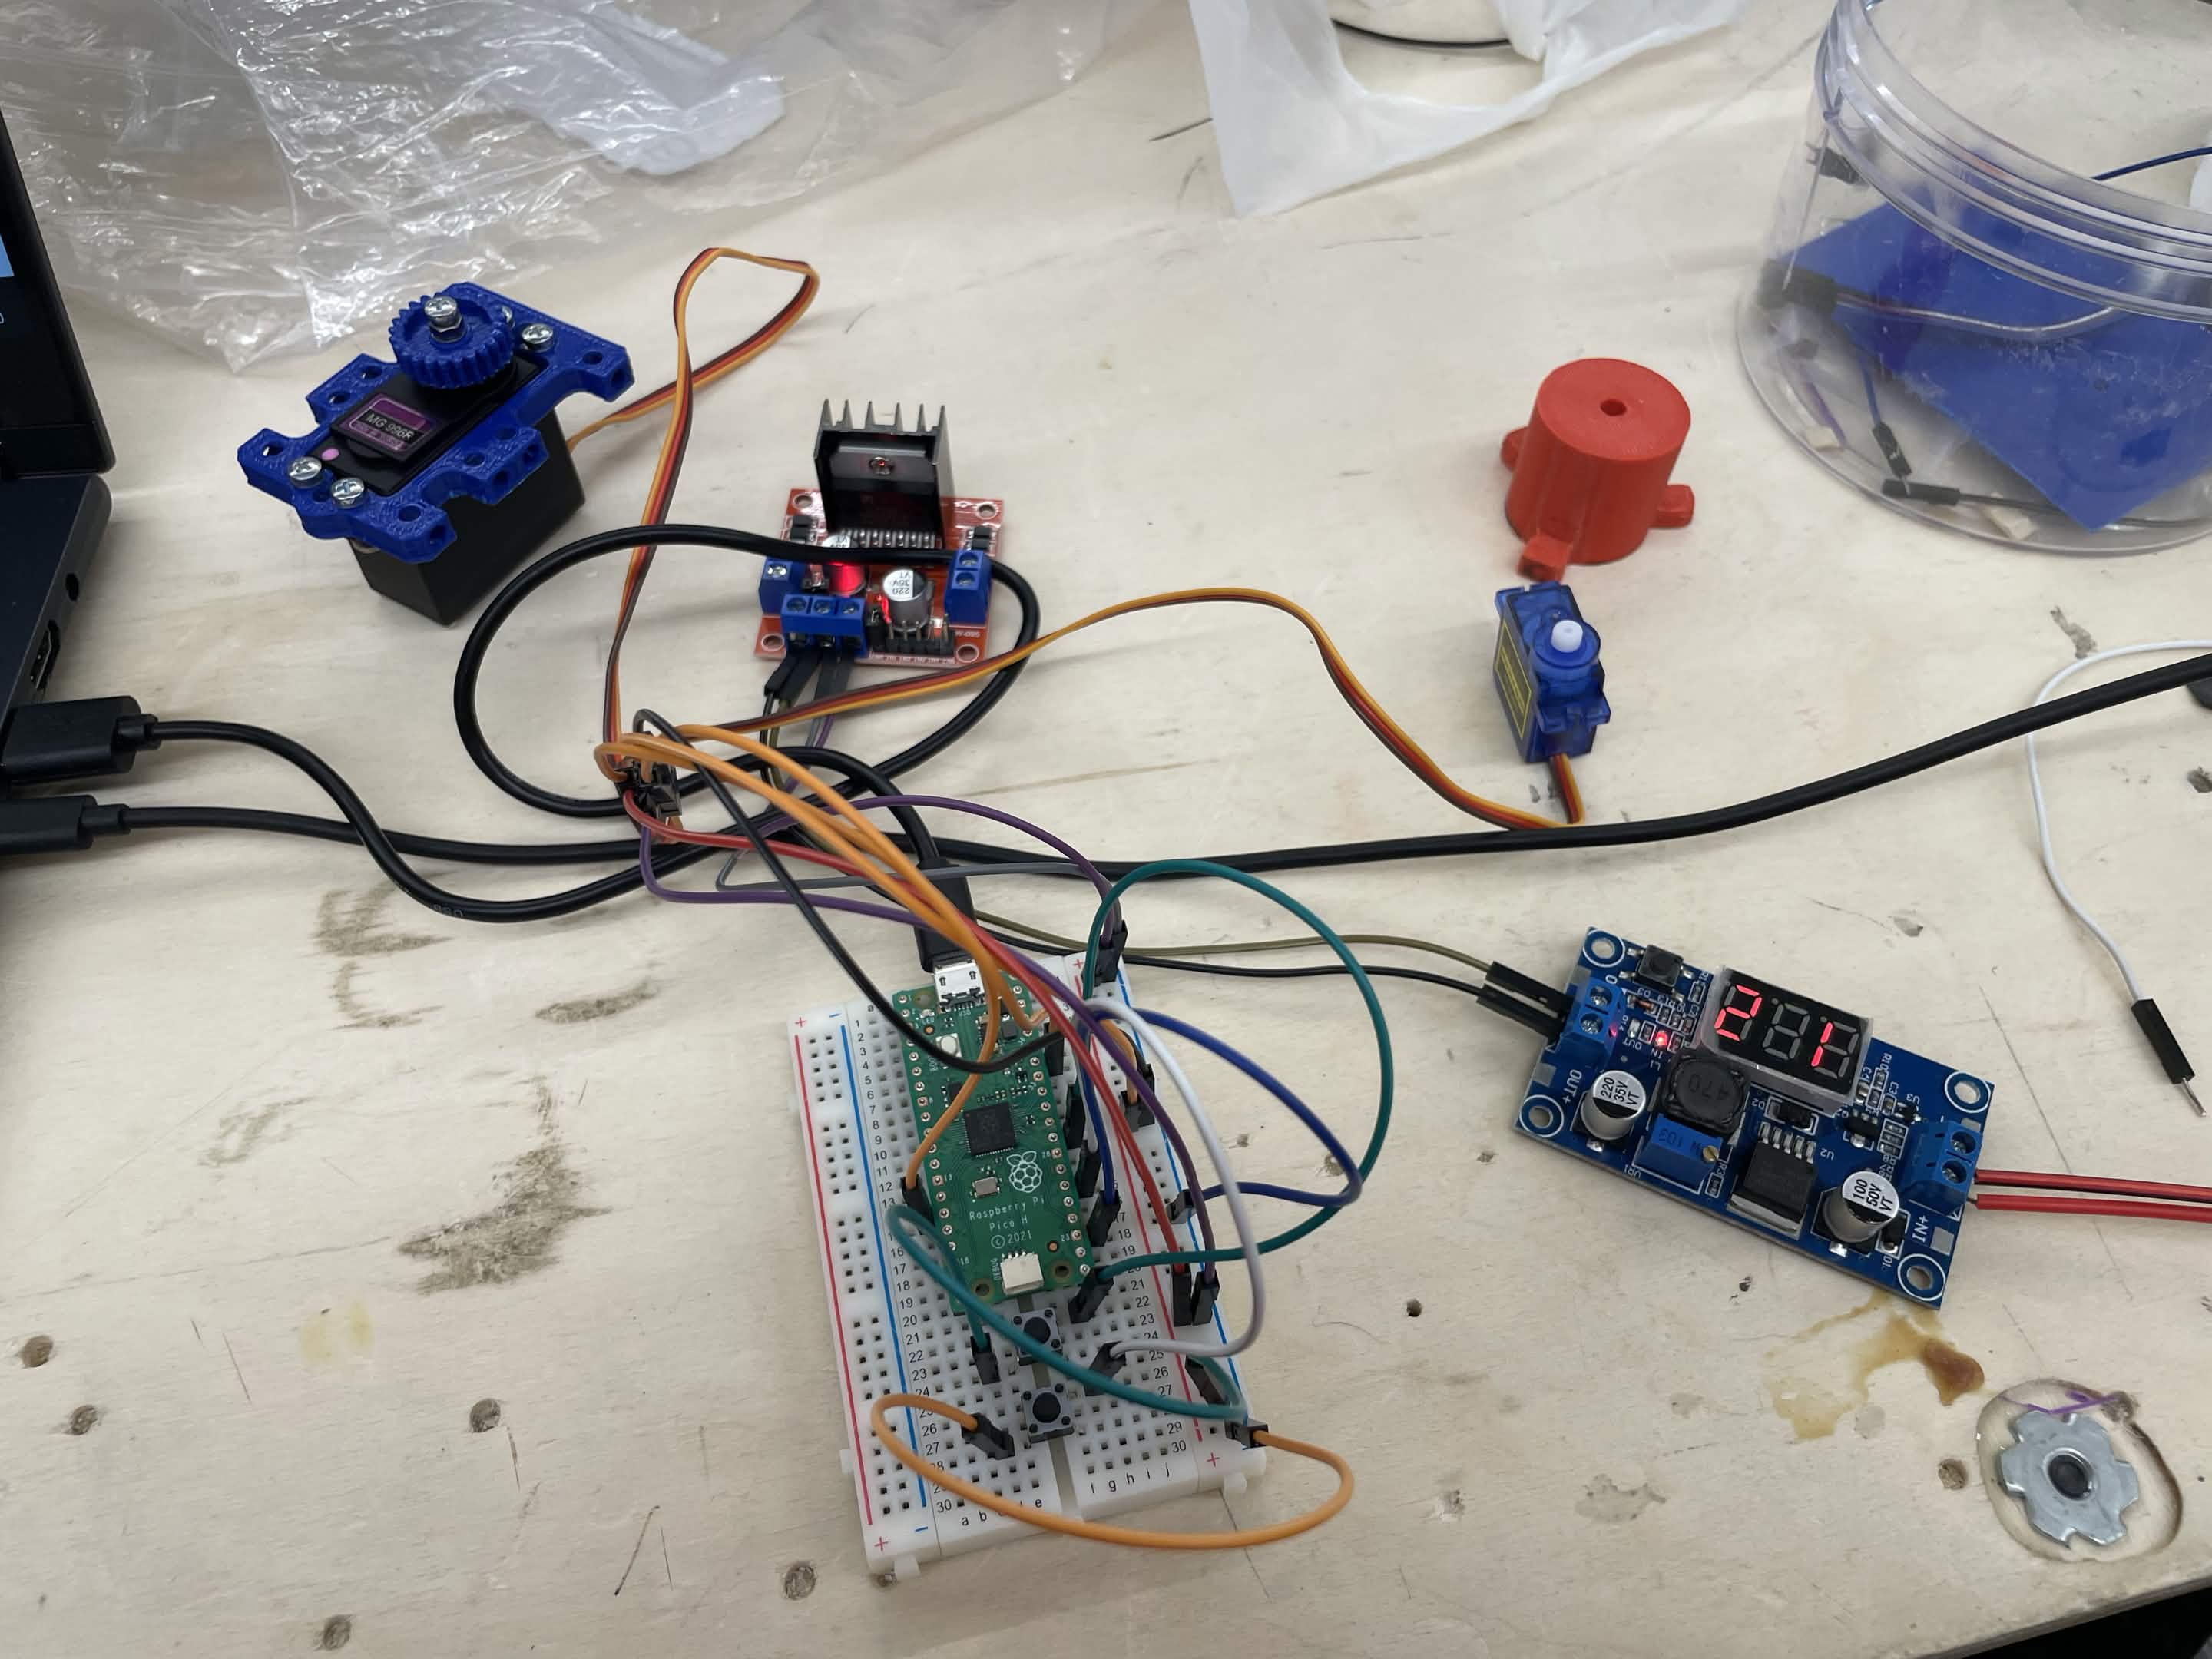
\includegraphics[width=0.75\textwidth]{../electrical_images/final_image.jpg}
\caption{Complete integrated circuit featuring two servo motors and two push button controls.}
\label{fig:final}
\end{figure}

\section{Conclusion}

The electrical circuit for the deployment system was successfully developed through a systematic build process. Starting from the Lab 3 foundation, the circuit was expanded to include proper power regulation, multiple servo motors, and user input controls. The final system provides a functional platform for testing and refining the deployment mechanism, with all electrical components properly integrated and operational.

\end{document}
